% What to use instead of masking. Numbers: results/round8/, results/round9/ (docs/PREREGISTRATION_ROUND8.md, ROUND9.md;
% stages/stage9_remedies_dominance), results/CROSS_COHORT.md and results/natural/*/natural_boot.json (label-free erasure,
% balancing on unaltered data). Figure: paper/figures/dominance.pdf (scripts/make_paper_round_tables.py).
\section{What to use instead of masking}\label{sec:guide}\label{sec:solution}
The location law says what masking cannot do. We therefore asked which remedy removes masking's in-ROI failure without
costing anything where masking already works, and registered the answer's criterion before testing it.

\paragraph{A class-conditional constraint on the masked features} Let $x$ be the frozen features of the masked image,
$y$ the diagnosis and $a$ the image-level artifact label produced by the automatic detectors of Sec.~\ref{sec:data},
used during training only. On the training images we compute the within-class mean differences
$\delta_y=\mu(x\mid a{=}1,y)-\mu(x\mid a{=}0,y)$, project the features onto the orthogonal complement of $\delta_0,\delta_1$
(or of their average; chosen on validation data) and fit an ordinary logistic head on all training images at their
natural weights. Within each class the head can then not score images with and without the artifact differently on
average: the shortcut's contribution, including that of the artifact's correlates, is removed along the directions the
data reveal, while no image is down-weighted. That matters because group balancing loses on unaltered data mainly
through the pairs whose two images share the artifact status, i.e.\ through disease evidence discarded by reweighting
(Supplement~S17). The constraint is the first-moment, linear case of counterfactual invariance
\citep{veitch2021counterfactual}; what is new here is its derivation from the location law and its use after masking. At
test time it needs only the masked image, like masking itself.

\paragraph{Registered test against masking} We registered a criterion for \emph{dominating} masking: not worse (margin
0.01 AUROC) on the six unaltered test sets and on the Trap~B and clean tests, better on every Trap~A and on the
conflicting pairs of the unaltered test sets, and no shortcut flipping --- 42 components, all of which must hold
(Supplement~S17). Settings were chosen per training set on validation data only (worst-group validation AUROC, with the
same-artifact validation AUROC kept within 0.005 of masking's, and masking as fallback); confirmation used trap resamples
generated after the registration and one cohort (ovary) that never influenced a choice. The constraint met 40 of 42
components (Fig.~\ref{fig:dom}). It is better than masking in every Trap~A --- thyroid $+0.330$ [$+0.311, +0.351$],
capsule $+0.153$ [$+0.131, +0.177$], dermoscopy hair $+0.193$ [$+0.166, +0.221$], held-out ovary $+0.118$
[$+0.089, +0.147$] --- and on the conflicting pairs of every unaltered test set (thyroid $+0.084$ [$+0.069, +0.101$],
ISIC 2020 $+0.078$ [$+0.069, +0.088$]); it is not worse on the Trap~B and clean tests and on four of the six unaltered
test sets, and it is inconclusive on the thyroid split ($-0.002$ [$-0.011, +0.007$]). Its one loss is ISIC 2020 overall
($-0.021$ [$-0.027, -0.016$]): there in-lesion hair still points to melanoma for most patients, and removing it costs on
those pairs. It covers the three regimes that separated earlier remedies: overlay-like calipers, pathology-like debris
and correlate-carried hair.
\ifdupfloats
\begin{figure*}[t]\centering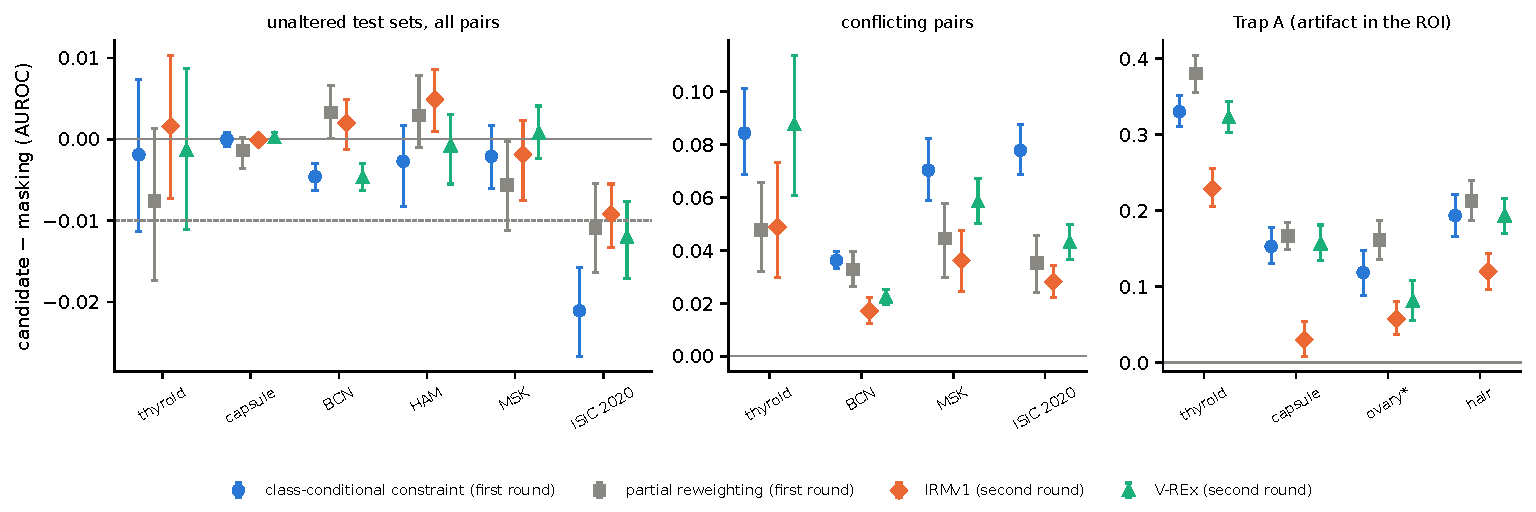
\includegraphics[width=\textwidth]{figures/dominance.pdf}
\caption{The four candidates closest to dominating masking, each minus masking (AUROC, crossed 95\% CIs), on the
confirmation data of their registered round (first round: class-conditional constraint, partial reweighting; second
round, on new resamples: IRMv1, V-REx). Left: all pairs of the unaltered test sets (dashed: the registered margin
$-0.01$). Middle: shortcut-conflicting pairs. Right: Trap~A, the worse of reversed and correlated AUROC; *ovary held out
from every choice.}\label{fig:dom}\end{figure*}
\fi

\paragraph{Nothing does better} A documented search over twelve further ideas on development data only --- backdoor
adjustment, product of experts and logit adjustment from language and long-tail learning, moment matching, conditional
adversarial debiasing, contrastive and invariance methods --- and a second registered round of its three best on new data
gave the same answer: IRMv1 met 41 of 42 components and lost only on ISIC 2020 overall ($-0.009$ [$-0.013, -0.005$]), and
the constraint, refitted with its frozen recipe, replicated its result (loss on ISIC 2020 only, $-0.015$
[$-0.024, -0.006$]). Every alternative to masking, including the unmasked model, loses overall on ISIC 2020 ($-0.009$ to
$-0.029$), mostly on pairs whose images share the artifact status: on new patients at natural prevalence masking is the
better disease ranker. No remedy we tested dominates masking.

\paragraph{Without artifact labels} When no artifact label is available, erasing from the frozen features the subspace
along which \emph{generic} synthetic overlays move the representation of masked images (mask-then-erase, U-MtE;
Supplement~S8) removes most of what masking leaves for overlay-like artifacts --- thyroid $+0.224$ [$+0.195, +0.253$] over
masking with DINOv2, $+0.246$ [$+0.224, +0.269$] with MedSigLIP and $+0.135$ [$+0.102, +0.168$] with a ConvNeXt --- but
it is worse than masking for debris that resembles the pathology ($-0.126$ [$-0.146, -0.107$]) and cannot reach a shortcut
carried by correlates: removing every hair patch with an oracle mask gains only $+0.015$. On the unaltered test
distributions no label-free remedy is uniformly better than masking: annotation-free U-MtE changes AUROC over masking by $-0.005$ [$-0.010, +0.000$] on capsule and $+0.007$ [$+0.005, +0.009$] for the held-out BCN hospital, its protected variant by $-0.023$ [$-0.027, -0.019$] on capsule, and group balancing by $-0.086$ [$-0.106, -0.067$] on capsule%
.

\paragraph{Decision guide} (i) Measure where artifacts sit relative to the ROI; for artifacts outside it, masking is
enough. (ii) For artifacts inside it, with image-level artifact labels from an automatic detector, use the
class-conditional constraint on the masked features, and expect a small overall cost where the deployment data still
reward the shortcut. (iii) Without artifact labels, U-MtE helps for overlay-like artifacts; for correlate-carried
shortcuts, which the oracle-removal ceiling on a handful of annotated images diagnoses, labels are needed. (iv) Evaluate
any remedy on shortcut-conflicting cases \emph{and} on the unaltered distribution, reporting clean, correlated and
reversed performance together, because a reversed-environment gain can be manufactured by removing diagnosis signal
(Supplement~S8).
